\section{Modeling --- Baseline Classifier (Logistic Regression)}

\subsection{Model Information}
Logistic Regression was selected as the Phase 1 baseline classifier which have:
\begin{itemize}
    \item \textbf{Interpretability:} Coefficients directly quantify each feature's contribution to the predicted default probability. This is valuable in credit risk contexts where explainability is often required.
    \item \textbf{Efficiency:} With $\sim$24,000 training rows and 35 features, Logistic Regression converges quickly and provides a reliable performance floor for comparison.
    \item \textbf{Class Imbalance Handling:} The \texttt{class\_weight='balanced'} parameter scales the per-sample loss function inversely with class frequencies, directly addressing the 78/22 imbalance.
    \item \textbf{Regularization:} Default L2 regularization shrinks redundant coefficients and reduces overfitting risk.
\end{itemize}

\subsection{Model Configuration}
The model was configured with the following parameters:

\begin{table}[h!]
\centering
\begin{tabular}{lll}
\toprule
\textbf{Parameter} & \textbf{Value} & \textbf{Justification} \\
\midrule
solver & lbfgs & Efficient quasi-Newton method; supports L2 penalty natively \\
max\_iter & 1000 & Ensures convergence without ConvergenceWarning on this dataset \\
class\_weight & balanced & Compensates for the 78/22 non-default/default split \\
random\_state & 42 & Matches Role 1 and Role 2 seeds for reproducibility \\
\bottomrule
\end{tabular}
\caption{Model Configuration Parameters}
\end{table}

\subsection{Training Pipeline}
The model was trained strictly on the training partition. The test set was never accessed during training to prevent data leakage. Figure 5 confirms the training and test dimensions after the full preprocessing pipeline. The training set contains 23,945 samples and 69 features, reflecting the one-hot encoding of all categorical variables (PAY\_0 through PAY\_6, EDUCATION, MARRIAGE, SEX). The 69-feature space is the result of the full ColumnTransformer pipeline applied by Role 1.

\begin{figure}[H]
  \centering
  
\includegraphics[width=0.9\textwidth]{sec3/image1.png}
  \caption{Training and test dimensions after preprocessing}
\end{figure}

\section{Performance Evaluation}

\subsection{Summary Metrics}
The trained model was evaluated on the held-out test set of 5,987 samples. Three primary metrics were computed:

\begin{table}[h!]
\centering
\begin{tabular}{lll}
\toprule
\textbf{Metric} & \textbf{Value} & \textbf{Interpretation} \\
\midrule
Accuracy & 76.83\% & Overall correct predictions --- less meaningful due to class imbalance \\
F1-Score (Default class) & 0.5162 & Primary metric --- harmonic mean of Precision and Recall for defaulters \\
ROC-AUC & 0.7634 & Model ranks a random defaulter above a non-defaulter 76\% of the time \\
\bottomrule
\end{tabular}
\caption{Summary Metrics}
\end{table}

\begin{verbatim}
              precision    recall  f1-score   support

Non-Default (0)       0.87      0.83      0.85      4661
Default (1)           0.48      0.56      0.52      1326

   accuracy                               0.77      5987
  macro avg           0.67      0.69      0.68      5987
weighted avg          0.78      0.77      0.77      5987
\end{verbatim}

\subsection{Confusion Matrix}
\textbf{Interpretation:} True Negatives (TN = 3,860) represent non-defaulting clients correctly cleared by the model. True Positives (TP = 740) are defaulters correctly flagged. The two error types are False Positives (FP = 801) --- non-defaulters incorrectly labelled as at-risk --- and False Negatives (FN = 586) --- defaulters the model failed to detect.
In credit-risk modeling, False Negatives carry the highest financial cost: a missed defaulter means the bank extends credit it will not recover. The FN count of 586 (representing 44\% of all actual defaulters in the test set) is the most critical limitation of this baseline and directly motivates the use of more powerful classifiers in the Final Deliverable. False Positives (801), while generating unnecessary credit reviews, carry a lower financial risk than FNs and are a manageable trade-off when using \texttt{class\_weight='balanced'}.

\begin{figure}[H]
  \centering
  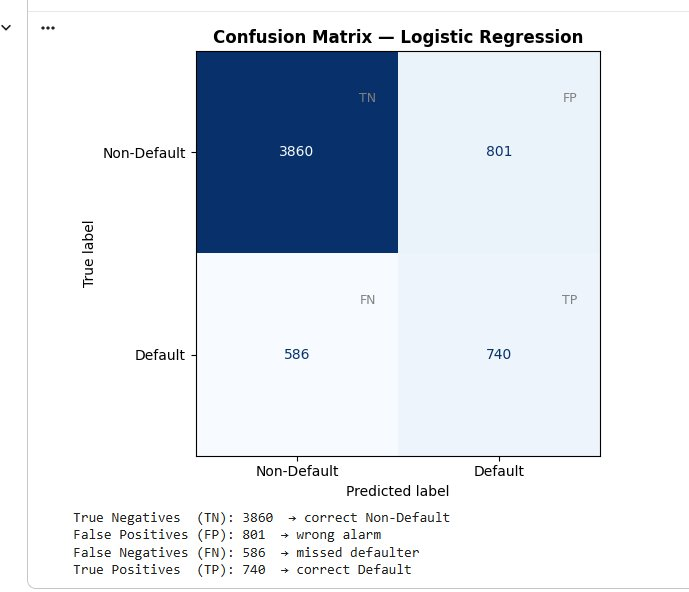
\includegraphics[width=0.72\textwidth]{sec3/image2.jpeg}
  \caption{Confusion matrix for Logistic Regression baseline}
\end{figure}

\subsection{ROC Curve}
Figure 8 presents the Receiver Operating Characteristic curve for the Logistic Regression model.

\begin{figure}[H]
  \centering
  
\includegraphics[width=0.82\textwidth]{sec3/image3.png}
  \caption{ROC curve of the baseline Logistic Regression model}
\end{figure}

\textbf{Interpretation:} The ROC curve plots the True Positive Rate (Recall) against the False Positive Rate at every classification threshold from 0 to 1. The shaded area under the curve (AUC = 0.763) indicates that the model correctly ranks a randomly selected defaulter above a randomly selected non-defaulter approximately 76\% of the time. This is significantly above the random baseline (AUC = 0.5, dashed line), confirming that the feature engineering and preprocessing pipeline introduced meaningful predictive signal. The steep initial rise of the curve at low False Positive Rates indicates that the model captures a substantial fraction of defaulters with few false alarms at higher decision thresholds. This shape suggests that threshold tuning (e.g., lowering the classification threshold from 0.5 to $\sim$0.3) could further improve Recall at an acceptable Precision cost --- a direction to be explored in Phase 2.

\subsection{Feature Coefficient Analysis}
Figure 9 displays the top 15 features ranked by the absolute value of their Logistic Regression coefficients.

\begin{figure}[H]
  \centering
  
\includegraphics[width=0.9\textwidth]{sec3/image4.png}
  \caption{Top feature coefficients by absolute magnitude}
\end{figure}

\textbf{Interpretation:} The coefficient chart confirms the findings of the EDA analysis. PAY\_0\_delay\_2\_months carries the largest positive coefficient ($\approx$ +1.25), making it the single strongest predictor of default --- consistent with the PAY\_0 bar chart in Section 4 which showed a dramatic increase in default rate for clients with a 2-month payment delay. PAY\_0\_delay\_3\_plus\_months ($\approx$ +0.90) ranks second, confirming that recent repayment delays are the dominant risk signal in this dataset. Among negative coefficients (features that reduce default risk), PAY\_2\_delay\_1\_month ($\approx$ -1.05) appears prominently --- suggesting that a one-month delay in an earlier billing period is associated with lower current default risk, possibly because such clients have since resolved their payment difficulties. EDUCATION\_others and PAY\_0\_no\_credit carry moderate negative coefficients, indicating that clients with non-standard education profiles or no credit history are less likely to default in this dataset. BILL\_AMT1 and PAY\_6\_revolving show small negative effects, consistent with the expectation that higher outstanding bills and revolving balances are not the primary default driver compared to repayment behaviour.
